\documentclass[11pt]{report}

\usepackage[T1]{fontenc}
\usepackage[polish]{babel}
\usepackage[utf8]{inputenc}
\usepackage{lmodern}
\usepackage[pdftex]{graphicx}
\selectlanguage{polish}
\usepackage{amsmath}
\usepackage[top=3cm, bottom=3cm, left=3cm, right=3cm]{geometry}
\usepackage{algorithm,algorithmic}
\title{Tytuł naszej pracy inżynierskiej}
\author{Katarzyna Śmietanka}
\begin{document}

%
% przeczytaj: http://en.wikibooks.org/wiki/LaTeX/Document_Structure
%

\maketitle
\tableofcontents

\chapter{Wstęp}

\section{Kontekst zagadnienia}

\par Problem układania planu zajęć dotyczy wielu instytucji głównie związanych ze szkolnictwem, od szkoły podstawowej aż to szkół wyższych. Zadanie sprowadza się do przygotowania graficznego rozkładu zajęć np. dla poszczególnych klas - uczniów uczęszczających do danej klasy, planu zajęć dla każdego z uczących nauczycieli oraz rozkładu zajęć dla każdej sali. Układanie planów zajęć nawet dla niewielkiej szkoły wymaga dużego wysiłku oraz nakładu czasowego. Problem staje jeszcze bardziej skomplikowany dla szkół ponadgimnazjalnych, do których uczęszcza więcej uczniów, tym samym jest więcej klas, nauczycieli oraz realizowanych przedmiotów. Ponadto zagadnienie ułożenia planu zajęć dla szkół wyższych, w których studenci mogą sami wybierać przedmioty w znacznym stopniu komplikuje te zagadnienie. Wynika to z tego, że aby dany plan zajęć był właściwy musi on spełniać podstawowe kryteria: dwa różne zajęcia na które jest zapisany minimum jeden student nie mogą się odbywać w tym samym czasie, dwa różne zajęcia w tym samym czasie nie mogą odbywać się w tej samej sali oraz nauczyciel w danym momencie może nauczać tylko jednego przedmiotu. Rozszerzeń tych ograniczeń jest wiele, a uwzględnienie każdego z nich, często konieczne do stworzenia realnego planu zajęć jest niezbędne. Wprowadzanie kolejnych ograniczeń znacznie utrudnia problem, który i tak jest stosunkowo skomplikowany.
\par Pomysł tematu pracy inżynierskiej wyniknął z przyglądania się na przestrzeni naszej edukacji planom zajęć które często odbiegały od idealnego według naszej opini. Plan zajęć często zawierał sporo przerw między obowiązkowymi zajęciami, zajęcia zaczynały się bardzo wcześnie lub kończyły bardzo późno, co w znacznym stopniu utrudniało powrót do domu bądź też dopasowanie innych poza uczelnianych zajęć do naszego planu.
\par Problem ułożenia planu zajęć podejmowany był w wielu pracach naukowych również na Politechnice Gdańskiej, co świadczy o tym że ułożenie bezkonfliktowego planu zajęć jest problemem stosunkowo trudnym do rozwiązania a zarazem bardzo ciekawym, ponieważ w bezpośredni sposób dotyczy każdej uczącej się osoby. Dlatego też na przestrzeni wielu lat powstało wiele różnych podejść do tego problemu od algorytmów klasycznych poprzez różnego typu algorytmy sztucznej inteligencji.
\par Problem układania graficznych rozkładów nie tylko związany jest ze szkolnictwem, ale również dotyczy konieczności ułożenia rozkładów jazdy komunikacji miejskiej \cite{com}
, planu zajęć dla pracowników \cite{worker} oraz terminarza zawodów sportowych \cite{sport}.
\section{Cel pracy}
\par Celem pracy jest zapoznanie się z problemem układania planów zajęć oraz przegląd różnych sposobów rozwiązania tego problemu. Jak również opracowanie, implementacja oraz porównanie działania wybranych przez nas algorytmów do układania planów zajęć : Algorytm roju cząsteczek (Particle Swarm Optimization), Algorytm Genetyczny (Genetic Algorithm) oraz Adaptacyjny Algotym Tabu (Adaptive Tabu Search). Stworzone algorytmy mają układać plan zajęć dla wyspecyfikowanego problemu, uwzględniając ograniczenia miękkie oraz ograniczenia twarde. 
\par Dodatkowo podjęliśmy się implementacji systemu w którym użytkownik będzie miał możliwość wygenerowania planu zajęć wybranym przez siebie algorytmem oraz wyświetlenia stworzonego planu zajęć w Google Calendar.
\par W ramach projektu planowane jest również dostosowanie realnych danych ze szkoly ponadgimnazjalnej do zaimplementowanych przez nas algorytmów.
\section{Zakres pracy}
\section{Podział zadań i obowiązków}
\chapter{Opis problemu układania planu zajęć}
\chapter{Specyfikacja problemu}
\section{Sformułowanie problemu}
\author{Katarzyna Śmietanka} \\
Celem jest stworzenie tygodniowego harmonogramu wykładów dla kilku kursów, z określoną liczbą dostępnych sal i przedziałów czasowych, w których mogą odbywać się zajęcia. Każdy wykład będący w programie danego kursu musi być przypisany do określonego przedziału czasu i sali tak by spełniał wejściowe ograniczenia. 
\subsection{Jednostki problemu}
\begin{itemize}
\item{\textbf{Dni, przedziały, okresy} - dzień podzielony jest na określoną liczbę przedziałów czasowych, okres para złożona z dnia i przedziału czasowego.}
\item{\textbf{Kursy i wykładowcy} - każdy kurs składa się z określonej liczby wykładów, które muszą być rozłożone w różnym czasie, na które uczęszcza określona liczna studentów i prowadzone są one przez wykładowcę. Dla każdego kursu jest określona minimalna liczba dni w których te wykłady muszą się odbyć, oraz okresy w których dane wykłady nie mogą się odbywać.}
\item{\textbf{Sale wykładowe} - sale wykładowe mają ograniczoną liczbę dostępnych miejsc w pomieszczeniu.}
\item{\textbf{Program nauczania} - składa się z kilku kursów, na które uczęszcza grupa studentów.}
\end{itemize}
\subsection{Ograniczenia}
\subsubsection{Ograniczenia twarde}
Plan jest wykonywalny - czyli możliwy do realizacji, jeżeli żadne z wymienionych poniżej ograniczeń nie jest naruszone.
\begin{itemize}
\item  ${H_{1}}$ \textbf{Wykłady} - każdy kurs wchodzący w skład programu nauczania musi być przypisany do różnego okresu.
\item  ${H_{2}}$ \textbf{Zajętość sali} - żadne dwa wykłady nie mogą odbywać się w tym samym okresie w jednym pomieszczeniu.
\item  ${H_{3}}$ \textbf{Konflikty pomiędzy kursami} - zajęcia z tego samego programu nauczania bądź nauczanie przez tego samego wykładowcę muszą odbywać się w różnym czasie.
\item  ${H_{4}}$ \textbf{Dostępność wykładowcy} - zajęcia nie mogą się odbywać w czasie, w którym dany wykładowca nie może prowadzić zajęć.
\end{itemize}
\subsubsection{Ograniczenia miękkie}
Ograniczenia te nie wpływają w bezpośredni sposób na wykonalność planu zajęć, ale na jego jakość uwzględniając poniższe kryteria, które wpływają na funkcję oceny wygenerowanego planu zajęć.
\begin{itemize}
\item  ${S_{1}}$ \textbf{Wielkość sali} - liczba studentów uczęszczajacych na zajęcia w danej sali musi być mniejsza bądź równa liczbie dostępnych miejsc.
\item  ${S_{2}}$ \textbf{Stabilność pomieszczenia} - zajęcia wchodzące w skład jednego kursu powinny odbywać się w jednej tej samej sali, jeżeli jest to niemożliwe liczba sal w których obdywają się te zajęcia powinna być jak najmniejsza.
\item  ${S_{3}}$ \textbf{Minimalna liczba dni} - minimalna liczba dni na które powinny być rozłożone zajęcia z danego kursu.
\item  ${S_{4}}$ \textbf{Zwartość zajęć} - zajęcia wchodzące w skład jednego kierunku powinny być w jak najmniejszych odstępach czasu pomiędzy sobą.
\end{itemize}
\subsection{Funkcja oceny}
\textbf{Ograniczenia twarde} - dla tego typu ograniczeń zliczane są podczas końcowej oceny poszczególne naruszenia ograniczań:\\
\begin{enumerate}
\item \textbf{Zajęcia / Wykłady} - naruszenie występuje w przypadku gdy zajęcia nie są przypisane do planu zajęć
\item \textbf{Zajętość sali} - naruszenie występuje gdy zostaną przypisane więcej niż jedne zajęcia do sali w tym samym czasie
\item \textbf{Konflikty} - naruszenie wystąpi wtedy gdy dwa zajęcia będące w konflikcie odbywają się w tym samym czasie (tzn. ci sami studenci uczęszczają na te zajęcia lub prowadzone są przez tego samego wykładowcę)
\item \textbf{Dostępność} - naruszenie występuje gdy zajęcia odbywają się w czasie, w którym niedostępny jest wykładowca 
\end{enumerate} 

\textbf{Ograniczenia miękkie} - zliczanie punktów kary
\begin{enumerate}
\item \textbf{Wielkość sali} - Jeżeli liczba studentów jest większa niż liczba dostępnych miejsc w sali to za każdego dodatkowego studenta punkt kary pomnożony przez współczynnik ${a_{1} = 1}$ 
\item \textbf{Minimalna liczba dni}
Jeżeli liczba dni podczas których odbywają się zajęcia jest mniejsza niż minimalna liczba dni w których powinny odbywać się zajęcia to do kary doliczamy rożnicę między minimalną liczbą dni a dni w których zajęcia się odbywają pomnożoną o współczynnik $a_{2} = 5$ 
\item \textbf{Zwartość zajęc}
Za każde zajęcia w planie należące do danego programu nauczania nieprzylegające do innych zajęć punkt kary pomnożony o współczynnik ${a_{3} = 2}$
\item \textbf{Stabilność pomieszczenia}
Te same zajęcia powinny odbywać się w jak najmniejszej liczbie różnych pomieszczań, za każde nowe pomieszczenie punkt kary pomnożony o współczynnik ${a_{2} = 1}$
\end{enumerate}

\subsection{Matematyczne sformułowanie problemu} \cite{tabu}
\par Na problem składa się ${n}$ kursów ${C = \{c_{1}, c_{2},...,c_{n}\}}$ które powinny być przydzielone do ${p}$ różnych okresów ${T = \{t_{1}, t_{2},...,t_{p}\}}$ oraz ${m}$ pomieszczeń w których mogą odbywać się zajęcia ${R = \{r_{1}, r_{2},...,r_{m}\}}$. Okres jest to para składająca się z dnia i przedziału czasowego (${d}$ - liczba dni a ${h}$ - liczba dziennych przedziałów czasowych, czyli ${p = d * h}$). Każdy z kursów składa się z ${n}$ zajęć ${L = \{l_{1},l_{2},...,l_{n}\}}$. Kursy wchodzą w skład ${s}$ programów nauczania ${CR = \{cr_{1}, cr_{2}, ..., cr_{s}\}}$, na program nauczania składają się kursy, na które uczęszczają ci sami studenci. 

\chapter{Opis zrealizowanych algorytmów}
\section{Adaptive tabu search}
\author{Tomasz Dziopa, Katarzyna Śmietanka}
\subsection{Specyficzne sformułowanie problemu}
\par Problem definiujemy w postaci macierzy ${X}$  rozmiaru ${p \times m}$ gdzie ${x_{i,j}}$ który definiuje przypisanie danych zajęć do ${t_{j}}$ okresu oraz sali ${r_{i}}$. Jeżeli w danym czasie w danej sali nie odbywają się zajęcia wartość ${x_{i,j}}$ będzie przyjmowała wartość ${null}$. Dzięki takiemu sposobowi zdefiniowania problemu nigdy nie zostanie naruszone ograniczenie twarde ${H_{2}}$ dotyczące zajętości sali.
\subsection{Ogólny opis algorytmu}
\par Opis zaimplementowanego przez nas algorytmu został zaczerpnięty z pracy ,,Adaptive TabuSearch for Course Timetabling'' \cite{tabu}
\par Na całość algorytmu składają się trzy fazy: faza inicjalizacji podczas której tworzony jest początkowy plan zajęć, przy pomocy zachłannej heurystyki, faza intensyfikacji, która jest właściwą fazą algorytmu Adaptive Tabu Search, której celem jest optymalizacja funkcji oceny ograniczeń miękkich. Końcowa faza - faza dywersyfikacji gdzie dokonywana jest redukcja naruszeń miękkich, tak aby nie łamać twardych ograniczeń. Na algorytm ten składa się wiele unikalnych cech między innymi struktury sąsiedztwa - podwójne łańcuchy Kempe, operator zaburzeń oraz dynamiczna integracja operacji przeszukiwania tabu z operatorem zaburzeń.

\subsection{Tabu Search}
\par Algorytm Tabu Search został zaprezentowany w 1986 roku przez Freda W. Glovera \cite{glover}. Jest to metaheurystyka, która opiera się na obserwacji, że proces przeszukiwania przestrzeni rozwiązań w poszukiwaniu najlepszego u ludzi i zwierząt opiera się na pamięci krótko- i długoterminowej. 
\par Pamięć krótkoterminowa realizowana jest w postaci listy ruchów zabronionych. W każdej iteracji przeglądamy strukturę sąsiedztwa w poszukiwaniu najlepszego rozwiązania. Sprawdzamy, czy ruch prowadzący do uzyskania najlepszego sąsiada nie znajduje się na liście ruchów zabronionych; jeżeli tak - rozważamy kolejnego najlepszego sąsiada, w przeciwnym wypadku - aktualizujemy rozwiązanie i dodajemy ruch prowadzący do niego jako ruch zabroniony.

\begin{algorithm}[H]
    \caption{Algorytm Tabu Search}
    \begin{algorithmic}
    \STATE{best = current}
    \WHILE{\emph{nie jest spełniony warunek stopu}}
    \STATE{sąsiedztwo = neighborhood(current)}
    \FOR{$i=0$ \TO len(sąsiedztwo)}
    	\IF{$ruch(current, sąsiedztwo[i]) \not \in lista\_tabu$}
    	\STATE $lista\_tabu = lista\_tabu \cup ruch(current, sąsiedztwo[i])$
    	\STATE current = sąsiedztwo[i]
    	\ENDIF
    \ENDFOR
    \ENDWHILE
    \end{algorithmic}
    \end{algorithm}

\subsection{Fazy algorytmu}
\subsubsection{Faza inicjalizacji}
\par W tej fazie tworzony jest wykonywalny plan zajęć czyli nienaruszający ograniczeń twardych ${H_{1} - H_{4}}$. W każdej iteracji wybierane jest jedno z zajęć z kursu i przypisywane do odpowiedniego okresu i pomieszczenia. Całość przydzielania odbywa się na podstawie dwóch heurystyk pierwsza z nich determinuje wybor kursu, który zostanie przypisany do planu zajęć oraz druga zaś określa parę okres-sala.
\par Dla każdego częściowo wykonywalnego planu zajęć ${P}$ (czyli takiego, do którego zostało przydzielone już część zajęć nie naruszając ograniczeń twardych) próbujemy wybrać jedne z zajęć z kursu, który posiada jeszcze nieprzydzielone zajęcia zgodnie z heurystyką ,,Wybór kursu''. Dzięki tej heurystyce uzyskujemy pierwszeństwo w przydzielaniu kursów mających małą liczbę dostępnych okresów do których może być przypisany oraz kursów z dużą liczbą nieprzypisanych zajęć do planu. Druga z heurystyk ,,Wybór okresu'' dotyczy wyboru okresu, do którego zostaną przypisane dane zajęcia. Celem jest wybór takiego okresu, który ma najmniejsze prawdobodobieństwo bycia wybranym w kolejnych krokach, dla kolejnych nieskończonych kursów.

\par \textbf{Oznaczenia}
\begin{enumerate}
\item $ lo_{i}(P)$ - liczba okresów do których mogą być przydzielone zajęcia z kursu $c_{i}$ dla planu ${P}$
\item $ lp_{i}(P)$ - liczba dostępnych par: okres- sala dla kursu ${c_{i}}$ dla planu ${P}$
\item $ lnz_{i}(P)$ - liczba nieprzydzielonych zajęć dla kursu ${c_{i}}$ dla planu ${P}$
\item $ lnk_{i, j}(P)$ - liczba zajęć z nieskończonych kursów, których nie można przydzielić do okresu ${t_{j}}$ po przydzieleniu jednego z zajęć z kursu ${c_{i}}$ do okresu ${t_{i}}$
\item $kom(i, j, k)$ - całkowita kara związana z ograniczeniami miękkimi po wykonalnym wstawieniu zajęć (tzn. nie naruszając ograniczeń $H1 - H4$ ) z kursu $c_{i}$ do okresu ${t_{j}}$ przydzieleniu sali ${r_{k}}$
\end{enumerate}
\par \textbf{Heurystyki}

\begin{enumerate}
  \item Wybór kursu 
  \begin{enumerate}
    \item Wybieramy kurs z najmniejszą wartością współczynnika:\\
     $ w_a(c_{i}) = \frac{lo_{i}(P)}{\sqrt{lnz_{i}(P)}}$
    \item Jeżeli istnieje więcej niż jeden kurs z tą samą wartością współczynnika ${w_a}$ wybieramy kurs z najmniejszym współczynnikiem \\ $ w_b(c_{i}) = lp_{i}(P) * \sqrt{lnz_{i}(P)} $
    \item Jeżeli istnieje więcej niż jeden kurs z tą samą wartością współczynnika $w_b$ to wybieramy kurs ${c_{i}}$ z maksymalną liczbą kursów współdzielonych kursów z tym kursem (tzn. mającym najwięcej konfliktów ze względu na studentów uczęszczających na ten kurs oraz uczących nauczycieli).
  \end{enumerate}
  \item Wybór okresu \\
  Dla każdej dostępnej pary (okres - sala) wybieramy parę z najmiejszą wartością funkcji $g(j, k) = K_{1} * lnk_{i,j}(P) + K_{2} * kom(i, j, k)$ \\
  $K_{1} = 1.0 $ - współczynnik związany z ograniczeniami twardymi \\
  $K_{2} = 0.5 $ - współczynnik związany z ograniczeniami miękkimi
\end{enumerate}



\subsubsection{Faza intensyfikacji}
\par W fazie intensyfikacji zostają wprowadzone struktury sąsiedztwa prostego oraz pojedyncze i podwójne łańcuchy Kempe, w obrębie tych struktur dochodzi do zamian poszczególnych zajęć tak by nie naruszyć ograniczeń twardych. Na algorytm Tabu Search składa się kombinacja połączenia zamian w obrębie tych dwóch struktur, które przeprowadzane są w cyklu token - ring. Celem tej fazy jest ograniczenie funkcji oceny ograniczeń miękkich, nie łamiąc żadnych ograniczeń twardych. Przestrzeń wykonywanych zamian dla poszczególnych zajęć jest ograniczona tylko do wykonywalnych zamian czyli takich, które po wykonaniu nie naruszają ${H1-H4}$.
\paragraph{Struktury sasiedztwa}
\begin{enumerate}
\item \textbf{Podstawowa struktura sąsiedztwa} \\
Jest to struktura, która zawiera wszystkie możliwe zamiany dla pary dwóch zajęć należących do różnych kursów i nie należących do tego samego okresu w planie zajęć. \\
Zamiana jest przypisaniem zajęć $x_{i_{1},j_{1}}$ w miejsce zajęć ${x_{i_{2}, j_{2}}}$ oraz zajęć ${x_{i_{2}, j_{2}}}$ w miejsce zajęć $x_{i_{1},j_{1}}$ \\
Możliwe przypadki zamian
\begin{enumerate}
\item Zamiana pomiędzy dwoma różnymi zajęciami należącymi do dwóch różnych kursów i okresów
\item Przypisanie zajęcia ${x_{i,j}}$ do wolnej pozycji - do okresu dla którego zajęcie ${x_{i,j}}$ nie wchodzi w konflikt z pozostałymi zajęciami w tym okresie (tzn. nie narusza ${H1-H4}$ )
\end{enumerate}
\textbf{Szczegóły implementacyjne}


\item \textbf{Zaawansowana struktura sąsiedztwa} 
\subparagraph{}
Jednym z klasycznych podejść do problemu układania planu zajęć jest podejście grafowe instancję problemu możemy przedstawić jako graf $G(V, E)$, gdzie wierzchołki grafu reprezentują kursy, a krawędzie reprezentują konflikty między kursami, który należy pokolorować na jak najmniejszą liczbę kolorów. 
\subparagraph{}Łańcuchy Kempe zostały zaproponowane jako narzędzie matematyczne, które miało służyć do udowodnienia twierdzenia o czterech kolorach. Mając dany graf $G$ i jego pokolorowanie na co najmniej dwa kolory, łańcuchy Kempe możemy zdefiniować jako maksymalne spójne podgrafy $G$, w których wszystkie wierzchołki mają nadany kolor $a$ lub $b$.
\subparagraph{}W naszym problemie łańcuchami Kempe będą maksymalne spójne podgrafy $G$, które zostały przypisane do okresu $i$ lub $j$. Dla łańcuchów $K_1$ i $K_2$, które zawierają maksymalne podgrafy kursów przypisanych do odpowiednio $i$ i $j$, gdzie $t_i$ i $t_j$ oznaczają wszystkie kursy przypasowane do $i$ i $j$, tworzymy nowe przypasowania:
\[ t_i' = (t_i \setminus  (K_1 \cup K_2)) \cup (t_j \cap (K_1 \cup K_2)) \]
\[ t_j' = (t_j \setminus  (K_1 \cup K_2)) \cup (t_i \cap (K_1 \cup K_2)) \]

Specjalnym przypadkiem jest, gdy jeden z łańcuchów jest pusty, wtedy:
\[ t_i' = (t_i \setminus K) \cup (t_j \cap K)\]
\[ t_j' = (t_j \setminus K) \cup (t_i \cap K)\]

Tak określony ruch można traktować jako rozszerzoną wersję podstawowej struktury sąsiedztwa, gdzie zamieniamy po kilka przypasowań na raz. Przy zamianie musimy uważać, aby nie wykonywać ruchów, które powodują przypasowanie większej liczby kursów, niż jest dostępnych sal. 

%- room assignment

\end{enumerate}

\subsubsection{Faza dywersyfikacji}
\par Jeżeli rozwiązanie nie może zostać poprawione za pomocą algorytmu tabu search uruchamiana jest trzecia faza - faza dywersyfikacji.Głównym jej elementem jest losowy operator zaburzeń mający na celu zniszczenie osiągniętego lokalnego minimum. Początkowo identyfikowane są zajęcia z wysoką karą wynikającą z funkcji oceny  i losowo wybierane są zajęcia dla których zostaną dokonane zamiany sprecyzowane w poprzedniej fazie.
\par W momencie zakończenia fazy intensyfikacji, poszczególne zajęcia ustawiane są w kolejności malejącej ze względu na wysokość funkcji oceny. Z puli $q$ pierwszych zajęć wybierane jest $n$ zajęć, gdzie zajęcie będące na $k$ miejscu w rankingu wybierane zgodnie z rozkładem prawdopodobieństwa $P(k) = k^{-4.0}$. Następnie dokonywane jest $n$ losowych zamian pomiędzy zajęciami (sprecyzowanych w fazie intensyfikacji), ale tylko takich które zawierają przynajmniej jedno z wybranych z rankingu zajęć. \\
\textbf{Szczegóły implementacyjne}
\section{Particle Swarm Optimization (PSO)}
\subsection{Ogólny opis algorytmu}
\par Opis zaimplementowanego algorytmu został zaczerpnięty z pracy ,,Timetable Scheduling Using Particle Swarm Optimization'' \cite{pso}
\par PSO jest metodą bazującą na zachowaniu społeczeństwa. Polega na przeszukiwaniu przestrzeni rozwiązań przy pomocy populacji (roju) rozwiązań kandydujących (nazywanych cząsteczkami). W każdej iteracji każde rozwiązanie kandydujące (cząsteczka) jest aktualizowane na podstawie dwóch najlepszych wartości. Pierwszą z nich jest poprzednia najlepsza pozycja k-tej cząsteczki w i-tej iteracji ${P}^{i}_{k}$. Drugą zaś jest globalna najlepsza pozycja spośród wszystkich cząsteczek ${G}^{i}$ zanotowana pomiędzy pierwszą a i-tą iteracją. Każda cząsteczka jest równoważna z kandydatem na rozwiązanie problemu. Cząsteczka prousza się zgodnie ze swoją prędkością, która bazuje na doświadczeniu owej cząsteczki oraz doświadczeniu innych cząsteczek. PSO zazwyczaj osiąga rozwiązanie bliskie optymalnemu w mniejszej liczbie iteracji niż algorytmy ewolucyjne czy genetyczne.  \subsection{Działaie algorytmu}
\subsubsection{Orginalna wersja}
\par Orginalne PSO można opisać w trzech krokach:

\begin{description}
  \item[Krok 1] \hfill \\
Liczba cząsteczek urzywana podczas rozwiązywania problemu jest ustalona z góry. Każda cząsteczka ma swoją własną pozycje, prędkość i najlepsze dotychczasowe rozwiązanie. Wtedy,
  \[f(P^{i}_{k}) \le f(P^{i-1}_{k}) \le \ldots \le f(P^{1}_{k})\].

  \item[Krok 2] \hfill \\
Proces aktualizacji prędkości jest realizowany jako:
\[V^{i+1}_{k} = V^{i}_{k} + C_{1} \cdot r_{1} \cdot (P^{i}_{k} - X^{i}_{k}) + C_{2} \cdot r_{2} \cdot (G^{i} - X^{i}_{k})\].
  \item[Krok 3] \hfill \\
Przemieszczenie się cząsteczki jest wykonywany przy pomocy poniższego równania:
\[X^{i+1}_{k} = X^{i}_{k} + V^{i+1}_{k}, i = 0,1,\cdots, M-1,\]
gdzie $M$ to rozmiar cząsteczki, $-V_{max} \le V^{i+1}_{k} \le V_{max}$ ($V_{max}$ to maksymalna prędkość), oraz $r_{1}$ i $r_{2}$ to zmienne losowe z zakresu $0 \le r_{1},r_{2} \le 1$. Jeśli rozwiązanie jest lepsze od $G^{i}$ to $G^{i}$ zostanie zastąpione przez lepsze rozwiązanie, żeby reprezentować $G^{i+1}$ w kroku 4. W przeciwnym razie, nie będzie żadnej zmiany w globalnym najlepszym wyniku i $G^{i} = G^{i+1}$. Te rekurencyjne kroki będą postępowały dopuki nie nastąpi jakiś warkunek stopu w kroku 5.  
\end{description}

\subsubsection{PSO w problemie układania planu}
\section{Genetic Algorithm}
\subsection{Ogólny opis algorytmu}
\par Algorytm genetyczny to rodzaj algorytmu przeszukującego przestrzeń alternatywnych rozwiązań problemu w celu wyszukania rozwiązań najlepszych. Obecnie zalicza się go do grupy algorytmów ewolucyjnych.
\par Algorytmy genetyczne zajmują bardzo ważne miejsce w dziedzinie projektowania i analizy algorytmów. Doskonale sprawdzają się w sytuacji, gdy problem, z którym przychodzi nam się zmierzyć, jest nie do rozwiązania w sposób klasyczny w sensownym czasie. Pozwalają znaleźć sub-optymalne rozwiązanie problemów, których dziedziny nie są łatwe do wyznaczenia. Są powszechnie stosowane tam, gdzie do uzyskania rozwiązania korzystamy z zagadnień sztucznej inteligencji oraz tam, gdzie uzyskanie rozwiązania jest bardzo złożonym problem, natomiast jego ocena jest łatwa i błyskawiczna.
\par Należy zaznaczyć, że algorytm genetyczny nie gwarantuje znalezienia rozwiązania optymalnego, lecz przybliżone. Istota jego działania jest zbliżona do charakterystycznych dla środowiska naturalnego procesów ewolucyjnych. Cały algorytm operuje na grupie (populacji) potencjalnych rozwiązań, których jakość (stopień, w jakim jest bliskie rozwiązania optymalnego) potrafimy ocenić i które zbliżają się w przypominającym ewolucyjny procesie do rozwiązania optymalnego.
\par Problem definiuje środowisko, w którym istnieje pewna populacja osobników. Każdy z osobników ma przypisany pewien zbiór informacji stanowiących jego genotyp, a będących podstawą do utworzenia fenotypu. Fenotyp to zbiór cech podlegających ocenie funkcji przystosowania modelującej środowisko. Innymi słowy - genotyp opisuje proponowane rozwiązanie problemu, a funkcja przystosowania ocenia, jak dobre jest to rozwiązanie. Genotyp składa się z chromosomów, gdzie zakodowany jest fenotyp i ewentualnie pewne informacje pomocnicze dla algorytmu genetycznego. Chromosom składa się z genów.
\par Najczęściej działanie algorytmu przebiega następująco:
\begin{enumerate}
\item Losowana jest pewna populacja początkowa.
\item Populacja poddawana jest ocenie (selekcja). Najlepiej przystosowane osobniki biorą udział w procesie reprodukcji.
\item Genotypy wybranych osobników są ze sobą kojarzone poprzez złączanie genotypów rodziców (krzyżowanie).
\item Przeprowadzana jest mutacja, czyli wprowadzenie drobnych losowych zmian.
\item Rodzi się kolejne pokolenie. Aby utrzymać stałą liczbę osobników w populacji te najlepsze (według funkcji oceniającej fenotyp) są powielane, a najsłabsze usuwane. Jeżeli nie znaleziono dostatecznie dobrego rozwiązania, algorytm powraca do kroku drugiego. W przeciwnym wypadku wybieramy najlepszego osobnika z populacji - jego genotyp to uzyskany wynik.
\end{enumerate}
\subsection{Historia i zastosowanie}
Sposób działania algorytmów genetycznych nieprzypadkowo przypomina zjawisko ewolucji biologicznej, ponieważ ich twórca John Henry Holland właśnie z biologii czerpał inspiracje do swoich prac. 
\subsection{Fazy algorytmu}
\subsubsection{Utworzenie rozwiązania początkowego}
\subsubsection{Selekcja}
\subsubsection{Krzyżowanie}
\subsubsection{Mutacja}
\subsubsection{Elityzm}
\subsection{Istniejące implementacje}
\chapter{Projekt systemu}
\subsection{Zastosowanie}
\subsubsection{Przypadki użycia}
\par
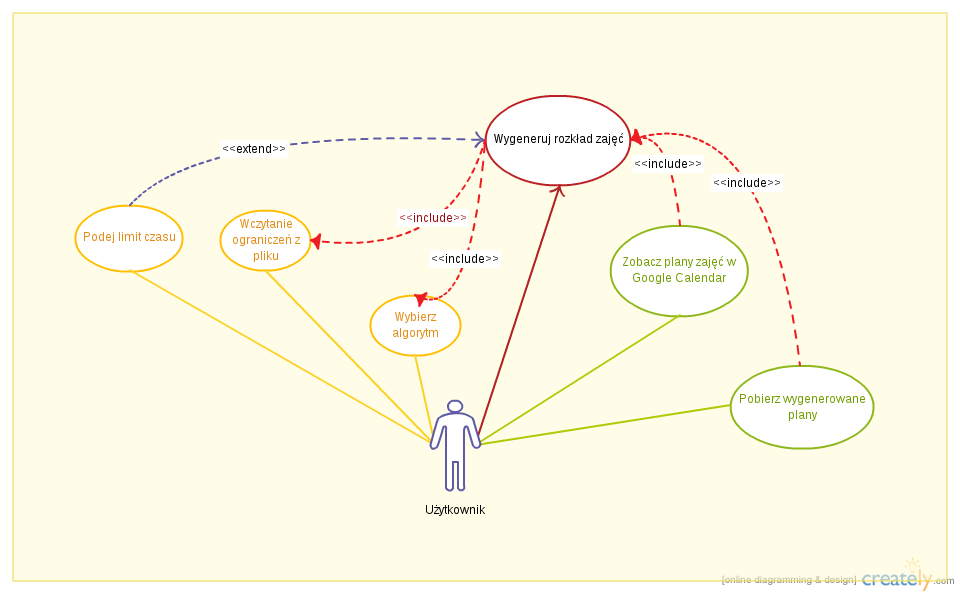
\includegraphics[width=0.8\textwidth]{InzynierkaUseCase.png}
\subsection{Architektura systemu}
\par
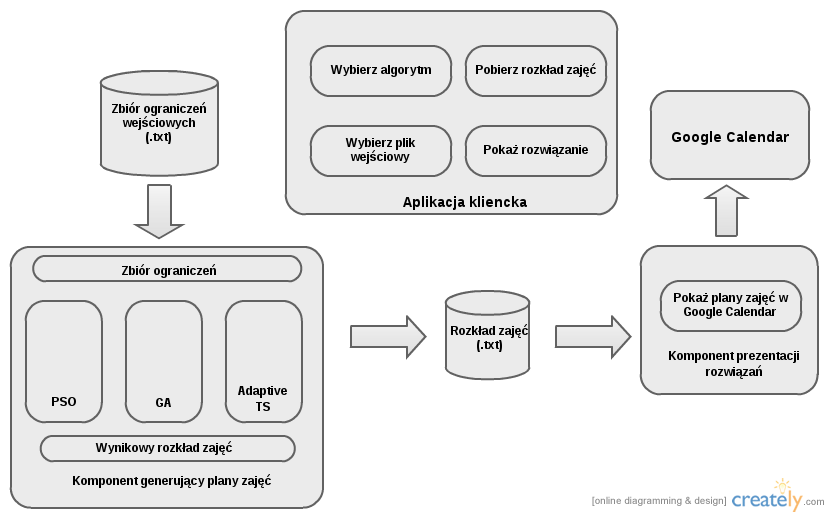
\includegraphics[width=0.8\textwidth]{ComponentsDiagram.png}
\chapter{Testy}
\chapter{Porównanie algorytmów}
\chapter{Sposób użytkowania systemu}
\chapter{Podsumowanie}

\begin{thebibliography}{2}
\bibitem{tabu} Zhipeng Lu, Jin-Kao Hao. Adaptive TabuSearch for Course Timetabling.  \emph{European Journal of Operational Research}, 200(1):235-244, 2010.
\bibitem{com} U. Brannlund, P. ). Lindberg, A. Nou, J. E. Nilsson. Timetabling using lagrangian relaxation Transportation Science 32, 358-369, 1998
\bibitem{sport} J. A. M. Schreuder. Constructing timetables for sport competitions. \emph{Mathematical Programming Study 13}, 58-67, 1980
\bibitem{worker} M. Chiarandini, A. Schaerf, F. Tiozzo. Solving employee timetabling problems with flexible workload using tabu search. \emph{Proceedings of the 3rd PATAT Conference}, 2013
\bibitem{pso} Autor1, Autor1. Tytuł.  \emph{European Journal of Operational Research}, 200(1):235-244, 2010.

\bibitem{glover} Fred Glover (1986). ,,Future Paths for Integer Programming and Links to Artificial Intelligence'' \emph{Computers and Operations Research}, 13 (5): 533–549.

\end{thebibliography}

\end{document}
